\documentclass{article}
\usepackage{graphicx}
\usepackage{amsmath}
\usepackage{setspace}
\usepackage[utf8]{inputenc}
\usepackage[T1]{fontenc}
\usepackage{xcolor}
\usepackage{placeins}
\usepackage{caption}
\usepackage[margin=1in]{geometry}
\usepackage{hyperref}
\usepackage{xcolor}
\usepackage[style=authoryear]{biblatex}
\addbibresource{ai_exposure.bib}

\title{An AI-Exposure Shock and Entry-Level Preferential Hiring Alternative}
\author{Ebba Mark \& Claude}
\date{}

\begin{document}

\maketitle
\doublespacing

\textcolor{red}{Note: Red text indicates the beginning and end of a section generated by Claude.}

\textcolor{blue}{Note: Blue text indicates either a reminder for Ebba to fix something/double-check Claude's work.}

\section{Overview}

This note describes our candidate alternative for the entry-level policy exercise. Previously, we applied a preferential hiring policy for long-term unemployed and entry-level workers during the simulation window (2001-2024). We will keep the LTU targeting design as it is (run the simulation from 2001-2024 with vs. without the policy), as it provides an interesting commentary on the Work Opportunity Tax Credit (WOTC). Essentially, we ask what could have been the effect of the WOTC if it had been applied effectively? We present this result in line with critiques of the WOTC.


In the original manuscript, we imposed preferential hiring for entry-level workers in the same way (compare 2001-2024 simulation with vs. without the policy). The below alternative takes a forward-looking (and likely more relevant) approach instead. We simulate the model from 2001-2024 without the policy, apply an AI-exposure shock at the end of our simulation period, either with or without the policy.
Essentially, rather than testing entry-level preferential hiring against
realised business-cycle conditions, it asks what the policy does in response to a hypothetical,
occupation-specific demand shock calibrated to recent evidence on AI exposure.

\section{Data}

\subsection{Occupational AI-exposure scores}

Occupation-level AI-exposure scores are drawn from \textbf{Eloundou, Manning, Mishkin \& Rock (2024)}, \url{https://www.science.org/doi/10.1126/science.adj0998}, which reports LLM-exposure ratings as exposure via direct LLM use plus complementary software) for 923 O*NET-SOC occupations.

\paragraph{Crosswalk.} The model's occupation network is coded in Census/ACS 2010
occupation codes (528 occupations). These are crosswalked to 2010 SOC detailed codes via
our preferred ACS-SOC crosswalk, then matched against
Eloundou et al.'s SOC codes. 361 of 528 occupations (68\%) match; of those, 345 (65\% of
all 528) retain a non-zero exposure score after min-max normalisation to $[0,1]$ -- the remaining 16
matched occupations' raw ratings equal the source's minimum and so normalise to exactly 0. Unmatched
occupations are
likewise assigned exposure $=0$, i.e. treated as unshocked. The result is a single exposure score per
occupation, $e_i \in [0,1]$.\label{par:crosswalk}

\begin{itemize}
\item \textcolor{blue}{Ebba to check cross-walk matching to see whether this can improve coverage. For now this crosswalks between 2018 and 2010 codes. I have a crosswalk for this somewhere to make sure it is consistent with other cross-walking we've done in the paper.}
\item \textcolor{blue}{Ebba to check the correlation between exposure shock and our own classification of occupations as entry-level. This will dictate whether we our entry-level hiring policy is effective/relevant here.}
\end{itemize}


\section{Method}

\subsection{Pre-Shock Initialization}
\label{sec:warmstart}

The shock is applied at the end of the simulated window (2024). Each model variant considered in this
note -- the three cross-model variants of Section~\ref{sec:crossmodel} and the full behavioural
reference model of Section~\ref{sec:single} -- is run under its own calibration window, from 2001-01
to 2024-05, for $N=10$ independent simulations, using that variant's own calibrated $\gamma_u$, $d_u$,
$\theta$ and behavioural flags. At the end of each run the live network state (every worker's
employment status, occupation, wage, and tenure, together with the vacancy pool) is captured. These
ten end-states are the starting points for the shock-phase runs below, for that variant.

Because the empirical demand series the calibration is built on ends in 2024, there is no real (read: currently downloaded) demand signal for the post-2024 period. Each occupation's target-demand multiplier is
therefore held at its calibrated no-shock value (1.0) going forward, except where reduced by the
imposed shock (Section~\ref{sec:shock}); the underlying \texttt{target\_demand} level itself (an
absolute headcount anchor used in the model's separation and vacancy-creation rules) is left at its
latest simulated value throughout. The real-world vacancy rate is held flat at its last observed value.

\subsection{Shock construction}
\label{sec:shock}

\textcolor{red}{Note: Claude's drafting contribution starts here.}

For each occupation $i$, the target-demand multiplier over the shock horizon $t = 0, \dots, 60$
months is

\begin{align}
  m_i(t) = 1 - \gamma \cdot e_i \cdot S(t)
\end{align}

where $e_i$ is the selected occupation's exposure score (Section~\ref{par:crosswalk}), $\gamma = 0.19$ is
the maximum fractional target demand reduction, anchored to the Brynjolfsson et al.'s estimate of the employment gap for young workers in AI-exposed occupations (the
paper's $\sim$19\% finding), and $S(t)$ is a logistic ramp normalised to run from exactly 0 at $t=0$
to exactly 1 at $t=60$, with midpoint at $t=30$ (half the horizon) and (\textcolor{blue}{uncalibrated!}) steepness $8/60$ months$^{-1}$.
Unexposed occupations ($e_i = 0$) are unaffected; the most exposed occupations see target demand fall
by up to 19\% by the end of the horizon \parencite{brynjolfsson_canaries_2025}.

\textcolor{red}{Note: Claude's drafting contribution ends here.}

\paragraph{Why $\gamma$ is needed.} $e_i$ measures technical, task-level exposure -- e.g. Eloundou et
al.'s rating reflects whether LLM assistance could plausibly cut the time needed for a task at equal
quality -- not a validated demand or employment elasticity. Time savings on a task do not mechanically
imply fewer workers are needed (firms may instead expand output), adoption is limited by cost and
integration frictions the score does not capture, and most occupations bundle exposed tasks with
non-exposed ones (oversight, judgement, interpersonal work) that still require the worker \parencite{eloundou_gpts_2024}. Applying
$e_i$ to target demand with $\gamma=1$ would assume technical exposure translates one-for-one into
demand destruction -- an assumption the exposure literature explicitly does not make. $\gamma=0.19$
instead keeps the shock's ceiling within what has actually been observed in the labour market
(the Canaries paper's employment gap for young workers in independently-identified AI-exposed
occupations), so $e_i$ sets which occupations are shocked and by how much \emph{relative to one
another}, while $\gamma$ sets the overall magnitude from real-world evidence rather than from the
exposure score's own scale.

Figure~\ref{fig:shock} shows the imposed shock itself: the target-demand multiplier $m_i(t)$, averaged
separately across the top quartile of occupations by exposure and the remaining three quartiles.

\begin{figure}[htbp]
  \centering
  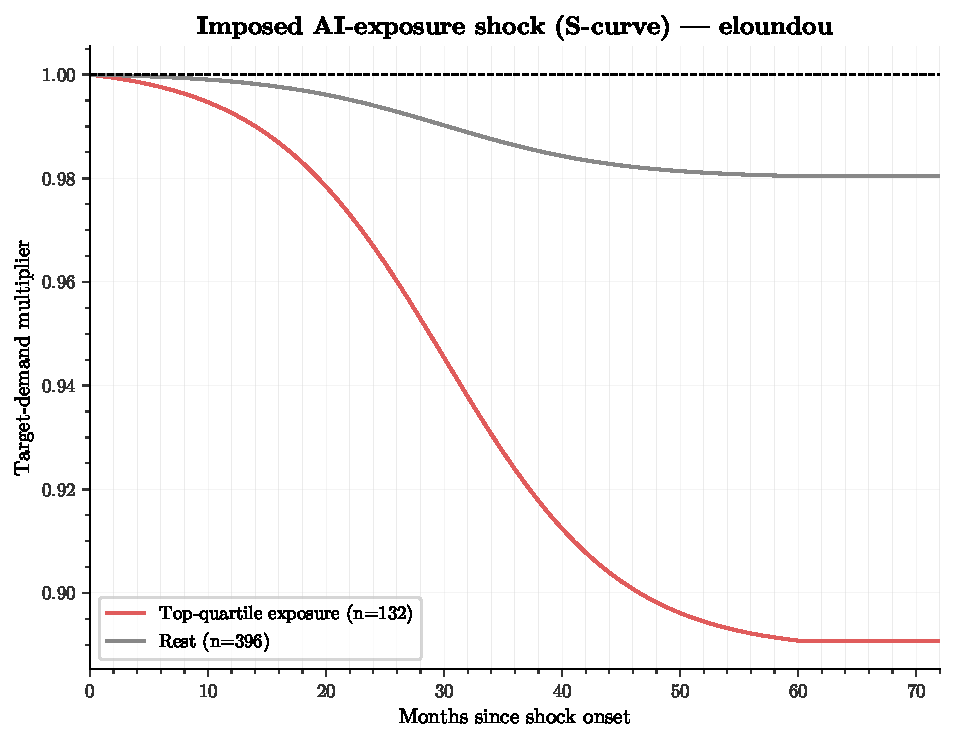
\includegraphics[width=0.8\textwidth]{eloundou/exposure_shock_implementation.pdf}
  \caption{The imposed AI-exposure shock (Eloundou et al. exposure score). Target-demand multiplier
  $m_i(t)$ over the 60-month shock horizon, averaged across occupations in the top quartile of exposure
  score versus the remaining three quartiles.}
  \label{fig:shock}
\end{figure}
\FloatBarrier

\subsection{Shock-phase runs}
\label{sec:shockphase}

From each of the ten end-of-simulation states, two 20-year (240-month) simulations are run under the
shock:

\begin{itemize}
  \item \textbf{No policy}: \texttt{entry\_hire\_bias} $=0$.
  \item \textbf{Policy}: \texttt{entry\_hire\_bias} $=1.0$ -- vacancies weight new-entrant applicants
  twice as heavily as other applicants when selecting a hire.
\end{itemize}

All other parameters (calibrated $\gamma_u$, $d_u$, $\theta$; behavioural flags; vacancy rule) match
the reference model's calibration. Because both scenarios for a given simulation start from the same
end-of-simulation states, comparisons below are paired at the simulation level. The S-curve itself
still fully ramps in over the first 5 years, exactly as in Section~\ref{sec:shock}.

\textcolor{red}{Note: Claude's drafting contribution starts here.}

Workers who enter the labour force during that 5-year ramp-in window are tagged, at creation, as a
lifetime-earnings cohort (Section~\ref{sec:lifetime} gives the full mechanics); everyone else is
excluded. Fifteen years of follow-up per cohort member was chosen as long enough for a policy-driven
earnings gap to emerge and compound well beyond what the near-term figures show, while still keeping
the shock-phase runs -- repeated for the reference model and all three cross-model variants -- within
reach computationally. Since the latest-arriving cohort member enters 5 years into the horizon, the
total simulated length is set to $20 = 15 + 5$ years so that \emph{every} cohort member, not just the
earliest arrivals, gets the same full 15-year follow-up; Figures~\ref{fig:crossmodel} and
\ref{fig:lifetime} both use this full 20-year horizon (tracking 15 years of follow-up per entrant for
the latter) -- all of it was already simulated and cached for the lifetime-earnings comparison, so
showing the full horizon in Figure~\ref{fig:crossmodel} too costs nothing extra.

\textcolor{red}{Note: Claude's drafting contribution ends here.}

\subsection{Cross-model comparison}
\label{sec:crossmodel}

To test whether the policy's effect depends on behavioural assumptions, the same warm-start and
shock-phase procedure is repeated independently for the same three model variants we currently use in the paper (non-behavioural benchmark, and two behavioural models without cyclical search with and without reservation wages). Each variant is simulated separately, using
its own 2001--2024 history.

Figure~\ref{fig:crossmodel} shows the policy's effect (policy minus no-policy) over the full 20-year
shock horizon for each of the three cross-model variants, for the unemployment rate and failed-hire
rate (Panels A-B, entry-level occupations only, matching the primary policy question), and, unlike
Panels A-B, computed across \emph{all} occupations so as to pick up spillover effects on the rest of
the economy that a purely entry-level metric would miss: the wage of every currently employed worker
(not just workers who were just hired as in Figure~\ref{fig:main}'s wage panel), shown two ways --
relative to each occupation's own median wage (Panel C), which isolates within-occupation pay changes
from any shift in which occupations people work in, and as a raw dollar level (Panel D), which bundles
both together and so is the more direct answer to whether the policy left the workforce better or
worse off in pay terms.

\begin{figure}[htbp]
  \centering
  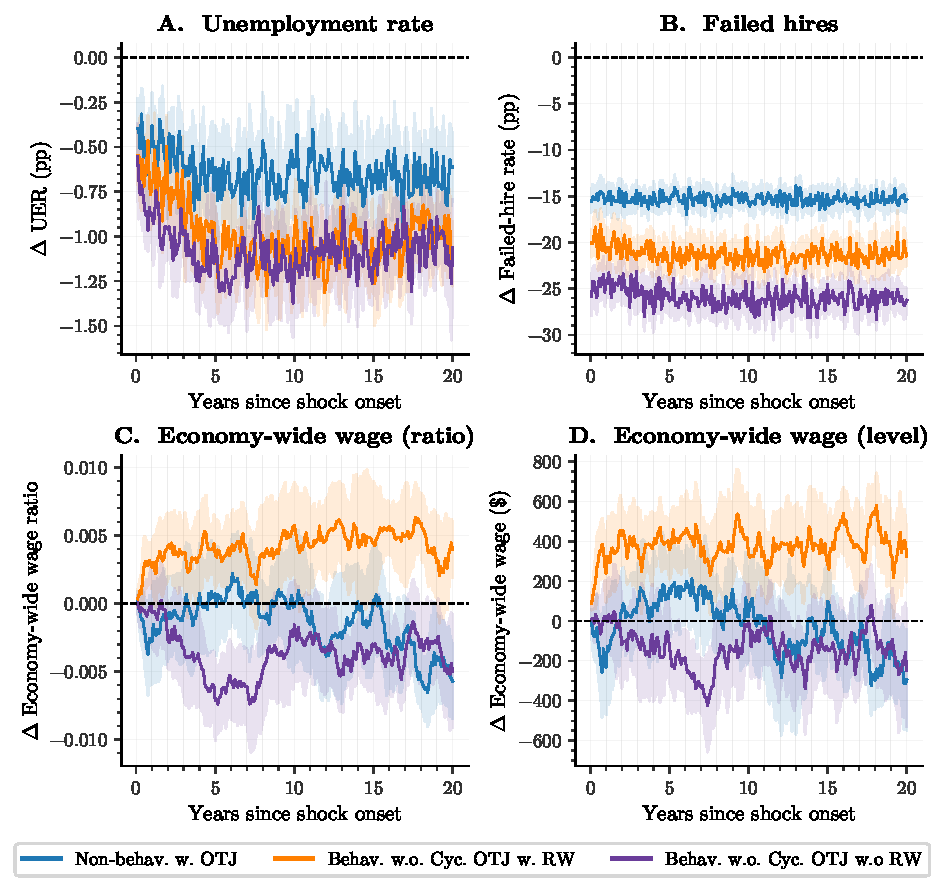
\includegraphics[width=\textwidth]{eloundou/fig_exposure_shock_cross_model.pdf}
  \caption{Robustness of the policy effect across behavioural model variants (Eloundou et al. exposure
  score), over the full 20-year (240-month) shock horizon. Each line shows the policy effect (policy
  minus no-policy), paired by warm-started simulation and averaged across $N=10$ simulations per
  variant. Panels A-B (entry-level occupations only):
  unemployment rate and failed-hire rate. Panels C-D (\emph{all} occupations, unlike A-B, so as to
  capture spillover effects on the rest of the economy): the wage of every currently employed worker in
  scope, not only new hires -- Panel C relative to each occupation's own median wage (isolating
  within-occupation pay changes), Panel D as a raw dollar level (which also reflects any compositional
  shift in which occupations people work in). Shaded bands show 95\% confidence intervals.}
  \label{fig:crossmodel}
\end{figure}
\FloatBarrier

\subsection{Lifetime earnings of entrants}
\label{sec:lifetime}

\textcolor{red}{Note: Claude's drafting contribution starts here.}

To ask whether the policy changes entrants' earnings over a longer horizon than the near-term figures
capture, we track a cohort of workers who enter the labour force during the shock's 5-year ramp-in
window (i.e. while the shock is actually being imposed) and follow their earnings for the 15 years
after the window closes. For each such worker, annual snapshots of wage are recorded; a year in which
the worker was unemployed at the snapshot date counts as \$0 earned that year rather than being
dropped, since excluding it would remove exactly the workers the policy is most likely to affect. Two
cumulative measures are tracked per worker: (i) each year's wage divided by the median annual wage of
the occupation the worker entered in -- fixed once at labour-market entry -- summed across years, and
(ii) raw annual wage in dollars, summed across years, with no normalisation.

% \textcolor{blue}{Note: the first version of this analysis divided each year's wage by the median wage
% of whatever occupation the worker currently held \emph{that year}, rather than the entry occupation.
% That produced two nearly indistinguishable curves. Diagnosing why: about 90\% of cohort workers hold
% more than one occupation over the follow-up window, and the occupations a worker moves between differ
% in median wage by a factor of $\sim$2$\times$ at the margin, so a moving denominator pulled the ratio
% back toward $\sim$1.0 every time a worker changed jobs -- masking real job-to-job earnings growth or
% decline rather than revealing it. Anchoring the denominator to the entry occupation (and, as a
% cross-check, tracking raw dollar earnings alongside it) fixes this.}

Because both the reference and cross-model shock-phase runs are warm-started from the same
end-of-2024 states (Sections~\ref{sec:warmstart}--\ref{sec:shockphase}), the comparison is paired at
the level of the warm-started simulation, exactly as in Section~\ref{sec:crossmodel}'s $\Delta$ figure.
Concretely, this collapsing happens in two stages, using two different summary statistics. First,
within a given simulation and scenario: each cohort worker's cumulative-earnings trajectory
(Section~\ref{sec:lifetime} above) is collapsed to the \emph{median} across every worker in that
simulation's cohort, at each year since entry -- giving one ``typical cohort member'' curve per
simulation, per scenario. The median (rather than the mean) is used here so that a handful of workers
with unusually large cumulative earnings -- e.g. an uninterrupted spell in a high-paying occupation --
do not dominate the per-simulation summary; with cohorts of hundreds to low thousands of workers per
simulation, the median is a stable, well-behaved statistic. Second, because policy and no-policy share
the same warm-started starting economy for a given simulation, we take the \emph{difference} between
that cohort median under the policy and under no-policy, within that same simulation, at each year;
this cancels simulation-specific variation in the warm-started economy rather than letting it compound.
Figure~\ref{fig:lifetime} plots the \emph{mean} of those ten paired differences (and their 95\% CI, from
the SEM across the ten simulations), under both measures, for the reference model -- the mean (not the
median) is used for this second, across-simulation step because $N=10$ is too small for a median to be
a stable or well-characterised estimator. So a given point on the figure is not an individual worker's
earnings gain -- it is the change in the entrant cohort's \emph{typical (median)} cumulative earnings,
averaged across ten independently warm-started economies.

% \textcolor{blue}{Note: both figures start at year 1, omitting year 0. At year 0 (the first annual
% snapshot, 0-6 months post-entry) roughly half the cohort has not yet found its first job, so the
% cross-sectional distribution of cumulative earnings is zero-inflated almost exactly at the 50th
% percentile. The median is discontinuous at that point: whether a given simulation's zero-share lands
% just above or just below 50\% (a coin-flip-level difference across simulations, confirmed against the
% underlying data) swings its year-0 median between exactly 0 and a real positive value, producing an
% artificial spike/drop between years 0 and 1 that reflects this threshold effect, not a real earnings
% difference. By year 1, over 97\% of the cohort has found employment at least once and the median is a
% stable statistic again.}

Figure~\ref{fig:crossmodel-lifetime} repeats the same procedure for each of the three cross-model
variants (Section~\ref{sec:crossmodel}), one line per model, styled identically to
Figure~\ref{fig:crossmodel}.

\textcolor{blue}{Note: this is \emph{not} an individual-level paired comparison. Because
\texttt{entry\_hire\_bias} changes how many random draws \texttt{hire()} consumes each period, the two
scenarios' shared random-number stream diverges, so which specific occupation each period's entrants
land in differs between the policy and no-policy runs even though the total number of entrants per
period is identical. The cohort \emph{definition} (arrival window, follow-up length) is the same across
both scenarios, and both start from the same warm-started economy, but individual entrants cannot be
matched one-to-one across scenarios.}

\textcolor{red}{Note: Claude's drafting contribution ends here.}

\begin{figure}[htbp]
  \centering
  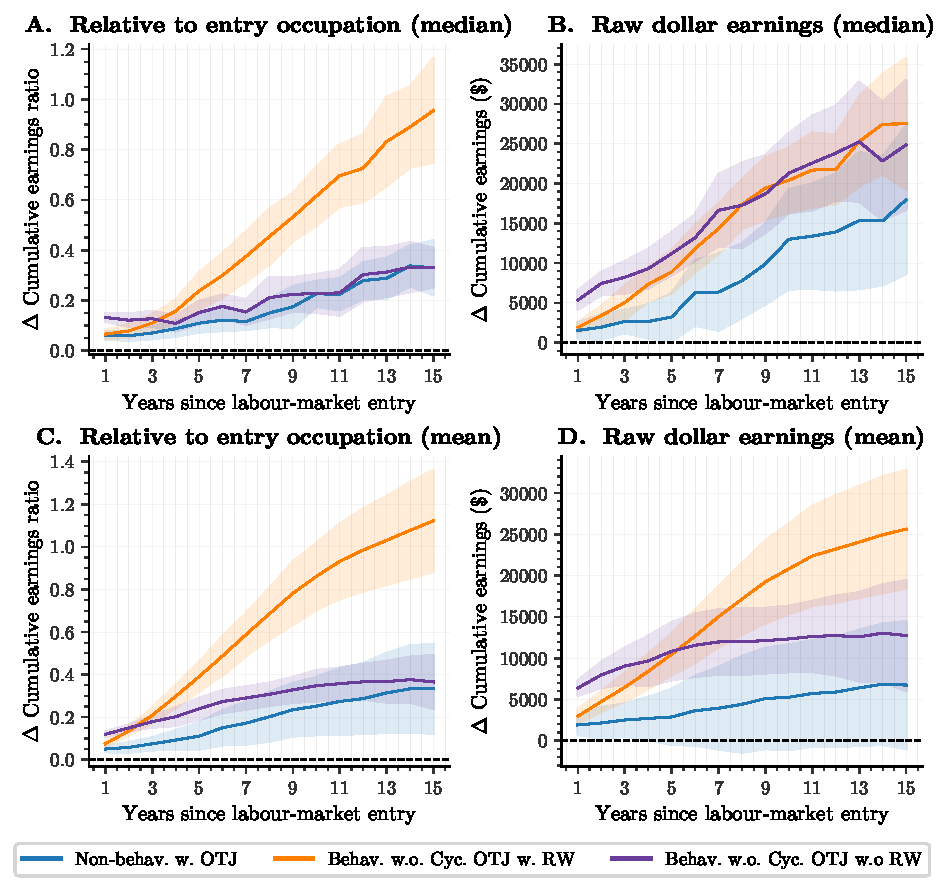
\includegraphics[width=\textwidth]{eloundou/fig_exposure_shock_cross_model_lifetime_earnings.pdf}
  \caption{Robustness of the lifetime-earnings effect (Figure~\ref{fig:lifetime}) across behavioural
  model variants (Eloundou et al. exposure score). Same cohort, follow-up window, and paired-$\Delta$-by-
  simulation procedure as Figure~\ref{fig:lifetime}, repeated independently for each of the three
  cross-model variants (Section~\ref{sec:crossmodel}), one line per model, coloured as in
  Figure~\ref{fig:crossmodel}. Top row (Panels A-B) uses the per-simulation cohort \emph{median}, the
  statistic used everywhere else in this note; bottom row (Panels C-D) repeats the same comparison using
  the per-simulation cohort \emph{mean} instead, shown purely as a robustness check on that choice.
  Panels A/C: $\Delta$ cumulative earnings relative to entry-occupation median wage. Panels B/D: $\Delta$
  cumulative raw dollar earnings. $N=10$ simulations per variant, shaded bands show 95\% confidence
  intervals.}
  \label{fig:crossmodel-lifetime}
\end{figure}
\FloatBarrier

\section{Single-Model Policy Effect}
\label{sec:single}

The reference model used in this section is our ``full behavioural model'' (cyclical OTJ search
intensity, concave search effort, and reservation wages) -- the specification used elsewhere in the
paper. It is warm-started and shock-tested using exactly the same procedure described in
Sections~\ref{sec:warmstart}--\ref{sec:lifetime}, but reported here on its own rather than alongside
the three cross-model variants of Section~\ref{sec:crossmodel}.

Figure~\ref{fig:lifetime} shows the lifetime-earnings comparison described in
Section~\ref{sec:lifetime}, for the cohort of entrants who arrive during the shock's ramp-in window,
tracked for the 15 years following that window: the policy effect (policy minus no-policy, paired by
simulation) under both measures -- cumulative earnings relative to entry-occupation median wage
(Panel A), and cumulative raw dollar earnings (Panel B).

Figure~\ref{fig:main} compares outcomes with (purple) and without (grey) the entry-level hiring policy, for
entry-level occupations (solid lines) and the rest of the economy (dotted lines): the unemployment
rate, first-job re-employment wages relative to the occupation median, the failed-hire rate (the share
of job offers that do not result in a hire), and
economy-wide UE and EE transition rates.

\begin{figure}[htbp]
  \centering
  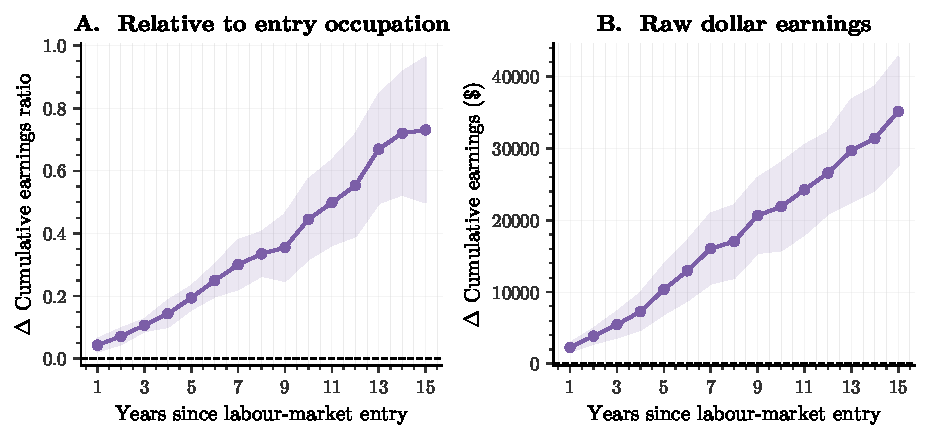
\includegraphics[width=\textwidth]{eloundou/fig_exposure_shock_lifetime_earnings.pdf}
  \caption{Lifetime-earnings effect of entry-level preferential hiring under the AI-exposure shock
  (Eloundou et al. exposure score): policy minus no-policy, paired by warm-started simulation. Cohort:
  workers who enter the labour force during the shock's 5-year ramp-in window, tracked for 15 years
  following that window. A year unemployed at the annual snapshot counts as \$0 that year. Panel A:
  $\Delta$ cumulative earnings relative to the worker's entry-occupation median wage (fixed at entry,
  not re-based on later occupation changes -- see Section~\ref{sec:lifetime}). Panel B: $\Delta$
  cumulative raw dollar earnings, no normalisation. Paired at the level of the warm-started simulation,
  not the individual entrant; $N=10$ simulations per scenario, shaded bands show 95\% confidence
  intervals.}
  \label{fig:lifetime}
\end{figure}
\FloatBarrier

\begin{figure}[htbp]
  \centering
  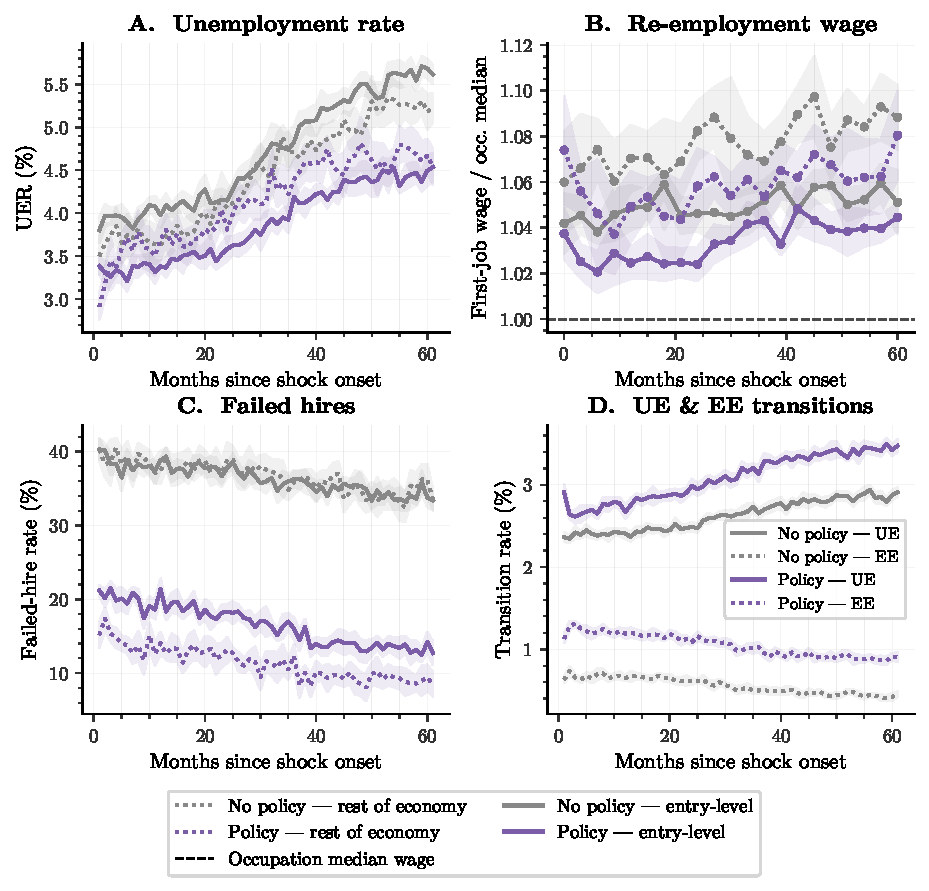
\includegraphics[width=\textwidth]{eloundou/fig_exposure_shock_entry_policy.pdf}
  \caption{Effect of entry-level preferential hiring under the AI-exposure shock (Eloundou et al.
  exposure score). Panel A: unemployment rate. Panel B: first-job wage relative to occupation median
  wage. Panel C: failed-hire rate. Panel D: economy-wide UE and EE transition rates. Solid lines:
  entry-level occupations; dotted lines (Panels A--C): rest of the economy. Grey: no policy; purple:
  entry-level preferential hiring. $N=10$ warm-started simulations per scenario; shaded bands show 95\%
  confidence intervals.}
  \label{fig:main}
\end{figure}
\FloatBarrier

\printbibliography

\end{document}
